\section{实验分析}
为了验证本章所提出的隐私保护神经网络框架的实用性,本节对本章的算法进行了实现。
%
我们基于Python的Numpy计算库~\cite{stefan_2011_numpy}实现了秘密分享的计算,其中秘密分享的整数环被选为$\mathbb Z_{2^{64}}$,因为64位整数能被计算机原生支持,可以方便地使用各种编程语言操作。
%
我们选择放缩系数为$2^{23}$,也就是对于任何实数(浮点数$x$),其整数表示为$x \cdot 2^{23}$。
此时定点数计算的精度达到$2^{-23}$,与32位浮点数的精确位一致~\cite{ieee_754_float},因此在该精度下神经网络的计算几乎不会有精度损失。
%
对于秘密分享中的通信交互,我们采用Python原生的套接字(Socket)接口进行编程,通过在节点之间建立持久化TCP连接的方式来交互数据,仅需初始化时的三次握手建立连接,防止其他上层协议带来的通信延迟。
同时我们采用流的方式进行数据读写,使用Pickle对变量进行打包。
%

\subsection{实验设置}
本节的实验在一台装备了16核Intel CPU,64GB内存的服务器上进行。
我们通过Linux自带的tc(Traffic Control)内核命令在本地网络(Localhost)上模拟了广域网(WAN, Wide Area Network)的带宽和延迟。
%
我们将WAN的带宽设置为80Mbps,将往返时间(Round Trip Time)设置为40ms。
%
这样的设置符合普通的家用宽带标准。
%
在实验开始之前,我们将训练数据以及初始化的神经网络权重秘密分享在$P_0$和$P_1$上。
%
我们对比了两个较新的密码学隐私保护神经网络方案,分别是SecureNN~\cite{wagh2019securenn}和ABY3~\cite{mohassel2018aby3}。
%
由于上述框架原始论文的开源代码未提供或无法运行,我们使用LatticeX-Rosetta库~\cite{latticex_rosetta}的SecureNN框架,以及TF-Encrypted库~\cite{tf_encrypted}的ABY3框架。
%
我们令所有的实验至少重复运行了10次,并把实验结果取平均值。


\begin{table}[h!]
\caption{逻辑回归的运行时间和通信量}
\label{tab:ss-perm:logistic}
\renewcommand{\arraystretch}{0.8}
\begin{tabular}{@{}cccrrrrrr@{}}
    \toprule
    \multicolumn{1}{l}{}     & \multicolumn{1}{l}{}    &    & \multicolumn{3}{c}{运行时间(秒)}       & \multicolumn{3}{c}{通信量(Mb)}       \\ 
    \cmidrule(lr){4-6}\cmidrule(lr){7-9}
    \multicolumn{1}{l}{输入维度} & \multicolumn{1}{l}{批大小} &    & 本方法            & SecureNN & ABY3  & 本方法            & SecureNN & ABY3  \\ 
    \cmidrule(lr){1-3}\cmidrule(lr){4-6}\cmidrule(lr){7-9}
    \multirow{4}{*}{100}     & \multirow{2}{*}{64}     & 推断 & \textbf{0.099} & 0.219    & 0.500 & \textbf{0.103} & 0.226    & 0.372 \\ \cmidrule(l){3-3}\cmidrule(lr){4-6}\cmidrule(lr){7-9}
        &                      & 训练 & \textbf{0.279} & 0.348 & 0.534 & \textbf{0.209} & 0.391 & 0.385          \\ \cmidrule(l){2-3}\cmidrule(lr){4-6}\cmidrule(lr){7-9}
        & \multirow{2}{*}{128} & 推断 & \textbf{0.108} & 0.228 & 0.500 & \textbf{0.202} & 0.448 & 0.624          \\ \cmidrule(l){3-3}\cmidrule(lr){4-6}\cmidrule(lr){7-9}
        &                      & 训练 & \textbf{0.281} & 0.367 & 0.539 & \textbf{0.413} & 0.775 & 0.639          \\ \midrule
    \multirow{4}{*}{1000}    & \multirow{2}{*}{64}     & 推断 & \textbf{0.132} & 0.358    & 0.511 & \textbf{0.996} & 1.072    & 1.369 \\ \cmidrule(l){3-3}\cmidrule(lr){4-6}\cmidrule(lr){7-9}
        &                      & 训练 & \textbf{0.294} & 0.698 & 0.831 & 1.988          & 2.581 & \textbf{1.678} \\ \cmidrule(l){2-3}\cmidrule(lr){4-6}\cmidrule(lr){7-9}
        & \multirow{2}{*}{128} & 推断 & \textbf{0.114} & 0.558 & 0.513 & 1.975          & 2.134 & \textbf{1.884} \\ \cmidrule(l){3-3}\cmidrule(lr){4-6}\cmidrule(lr){7-9}
        &                      & 训练 & \textbf{0.334} & 1.202 & 0.837 & 3.949          & 5.121 & \textbf{3.225} \\ \bottomrule
\end{tabular}
\end{table}

\begin{table}[h!]
\caption{神经网络的运行时间和通信量}
\label{tab:ss-perm:dnn}
\renewcommand{\arraystretch}{0.8}
\centering
\begin{tabular}{@{}cccrrrrrr@{}}
    \toprule
    \multicolumn{1}{l}{}  & \multicolumn{1}{l}{} &    & \multicolumn{2}{l}{运行时间(秒)} &      & \multicolumn{2}{l}{通信量(Mb)} &       \\ \cmidrule(lr){4-6}\cmidrule(lr){7-9}
    \multicolumn{1}{l}{模型} & \multicolumn{1}{l}{批大小} &    & 本方法           & SecureNN & \phantom{12}ABY3 & 本方法            & SecureNN & \phantom{12}ABY3           \\ \cmidrule(lr){1-3}\cmidrule(lr){4-6}\cmidrule(lr){7-9}
    \multirow{4}{*}{DNN1} & \multirow{2}{*}{64}  & 推断 & \textbf{0.19}     & 0.68    & 0.75 & \textbf{0.39}     & 1.98    & 1.90  \\ \cmidrule(l){3-3}\cmidrule(lr){4-6}\cmidrule(lr){7-9}
                            &                         & 训练 & \textbf{0.54} & 1.29     & 0.88 & \textbf{0.78}  & 4.05     & 2.21  \\ \cmidrule(l){2-3}\cmidrule(lr){4-6}\cmidrule(lr){7-9}
                            & \multirow{2}{*}{128}    & 推断 & \textbf{0.20} & 1.10     & 0.92 & \textbf{0.70}  & 3.89     & 3.63  \\ \cmidrule(l){3-3}\cmidrule(lr){4-6}\cmidrule(lr){7-9}
                            &                         & 训练 & \textbf{0.59} & 2.08     & 1.78 & \textbf{1.38}  & 7.90     & 4.10  \\ \midrule
    \multirow{4}{*}{DNN2} & \multirow{2}{*}{64}  & 推断 & \textbf{1.05}     & 5.67    & 1.86 & \textbf{10.69}    & 25.18   & 17.16 \\ \cmidrule(l){3-3}\cmidrule(lr){4-6}\cmidrule(lr){7-9}
                            &                         & 训练 & \textbf{1.86} & 12.11    & 3.24 & \textbf{17.97} & 55.98    & 35.20 \\ \cmidrule(l){2-3}\cmidrule(lr){4-6}\cmidrule(lr){7-9}
                            & \multirow{2}{*}{128}    & 推断 & \textbf{1.26} & 9.88     & 3.65 & \textbf{12.54} & 43.08    & 36.09 \\ \cmidrule(l){3-3}\cmidrule(lr){4-6}\cmidrule(lr){7-9}
                            &                         & 训练 & \textbf{2.58} & 20.00    & 5.14 & \textbf{24.84} & 93.19    & 47.71 \\ \bottomrule
\end{tabular}
\end{table}


\subsection{基准测试}
我们在逻辑回归模型以及全连接神经网络上对本方法和SecureNN~\cite{wagh2019securenn}、ABY3~\cite{mohassel2018aby3}框架进行了效率的评估,包含了运行时间、网络通信量的测量。

\textbf{逻辑回归}:
对于逻辑回归模型,我们把输入维度设置为100或1000,并把样本批次大小(Batch Size)设置为64或128。
实验结果汇报在\ref{tab:ss-perm:logistic}中。
可以看出,本章提出的方法相比于对比方法,训练或推断用时减少了2 -- 4倍,并且在大多数情况下也取得了更低的通信消耗。
%



\textbf{神经网络}:
我们测试了两种全连接神经网络模型,其输入维度分别为100和1000,云层大小分别为50和500。
样本批次大小也同样设置为64和128。
实验结果汇报在\ref{tab:ss-perm:dnn}中。
%
实验结果表明,相比于逻辑回归模型,本方法在神经网络上具有更高的优越性。
本方法相比于对比方法,在训练速度上有1.5 -- 5.5倍提升,同时减少了40\% -- 80\%的通信量。
这是因为神经网络的计算中有更多的非线性激活函数计算,使得本方法更多地发挥了在激活函数上的优势。
%



%
\begin{figure}[h!]
    \centering
    \begin{subfigure}[b]{0.48\linewidth}
    \centering
    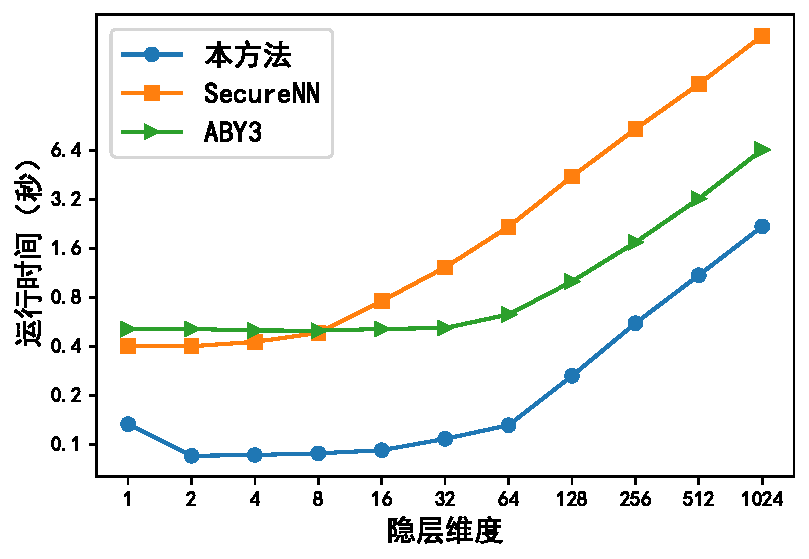
\includegraphics[width=\linewidth]{Z_Resources/ss-perm_one-layer-time.pdf}
    \caption{运行时间}
    \end{subfigure}
    %
    \begin{subfigure}[b]{0.48\linewidth}
    \centering
    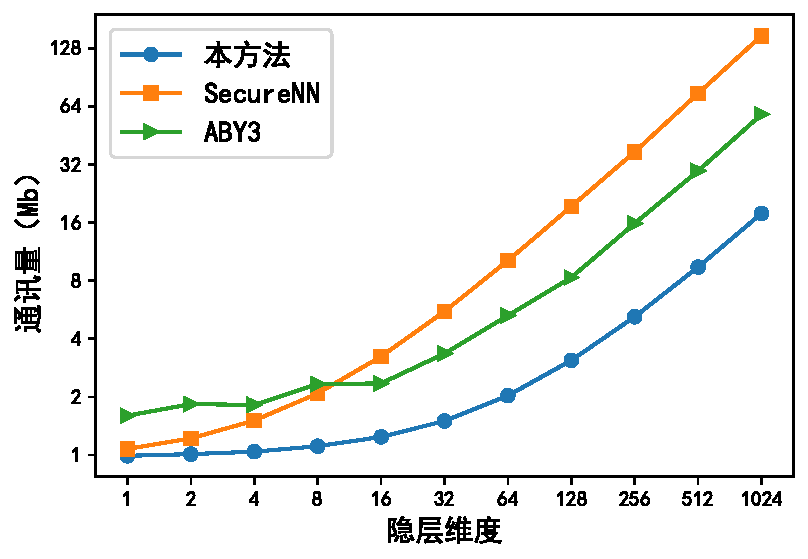
\includegraphics[width=\linewidth]{Z_Resources/ss-perm_one-layer-comm.pdf}
    \caption{总计通信量}
    \end{subfigure}
    
    \begin{subfigure}[b]{0.48\linewidth}
    \centering
    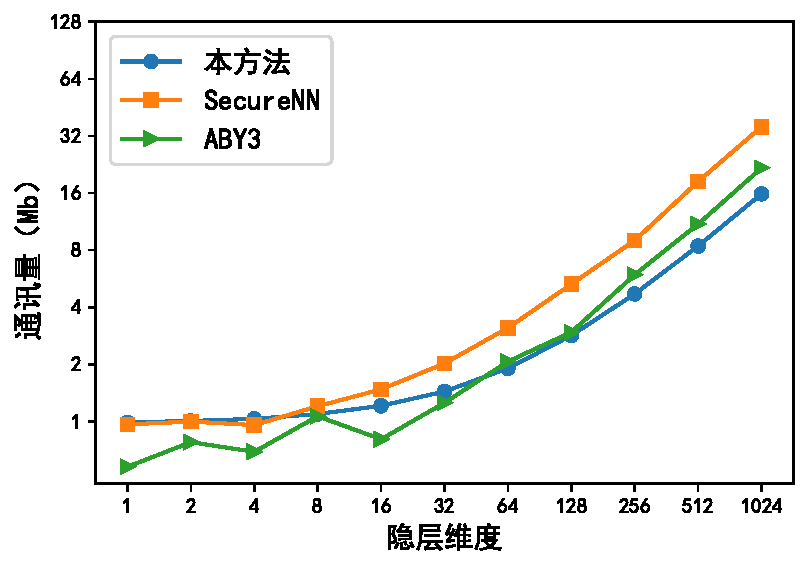
\includegraphics[width=\linewidth]{Z_Resources/ss-perm_one-layer-c01.pdf}
    \caption{$P_0$和$P_1$之间的通信量}
    \end{subfigure}
    %
    \begin{subfigure}[b]{0.48\linewidth}
    \centering
    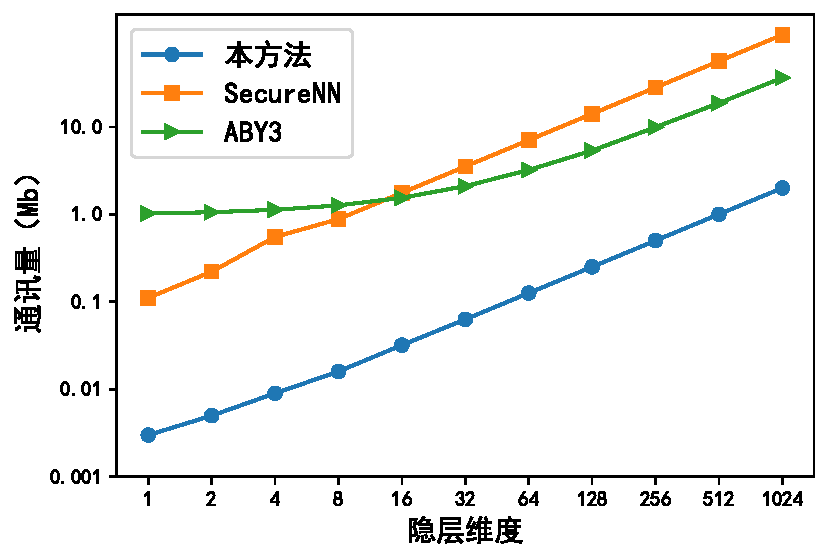
\includegraphics[width=\linewidth]{Z_Resources/ss-perm_one-layer-c2.pdf}
    \caption{$P_2$的通信量}
    \end{subfigure}
\caption{不同隐层维度时的运行时间和通信量}
\label{fig:ss-perm:layer-dim}
\end{figure}

\subsection{隐层维度对开销的影响}
为了测试本方法在不同大小的隐层上的效果,本节对本方法和对比方法在不同大小的神经网络隐层的运行时间以及通信量进行了测试,其中隐层的输入维度固定为1000。
%
本实验不仅测试了总计通信量,也测试了$P_0$和$P_1$之间的通信量和$P_2$相关的通信量。
%
实验结果呈现在\ref{fig:ss-perm:layer-dim}中。
%
可以看出,随着隐层维度逐步增加,本方法的优势逐渐扩大。
当隐层维度达到64左右时,本方法的所有通信量指标都是最低的。
%
本方法尤其减少了辅助第三方($P_2$)的通信量,相比于其他方法的通信量减少了大概1个数量级。
由于三种方法均采用秘密分享进行线性运算,因此$P_0$和$P_1$之间的通信量差距较小。

\subsection{真实数据集实验}
为了测试本章提出的方法在实际场景下的效果,本节对本章方法在真实数据下进行了实验,并且将其和明文训练进行对比,考察了训练准确率以及隐层经过随机排列后的隐私泄露程度。

\subsubsection{准确率}
为了验证本方法的训练准确率,我们在Gisette数据集~\cite{2008_gisette}和MNIST数据集~\cite{mnist}上分别使用本方法进行模型训练,同时与明文对比,并绘制出验证集准确率随着训练轮数变化的曲线图,呈现在\autoref{fig:ss-perm:train}a-c中。

%
Gisette数据集~\cite{2008_gisette}是一个二分类数据集,包含了6000个训练样本和1000个测试样本,特征维度为5000。
我们用逻辑回归模型对其进行了训练。
%
MNIST数据集~\cite{mnist}是一个10分类的手写数字分类数据集,包含了60000个训练样本和10000个验证样本。
我们用两个全连接神经网络(DNN1、DNN2)对其进行训练,其结构分别为784-128-10和784-128-32-10,DNN2的第一个隐层激活函数为ReLU,其余隐层采用Sigmoid作为隐层激活函数。

实验结果表明,采用本方法的隐私保护逻辑回归和神经网络的训练曲线与明文神经网络的训练曲线几乎重合,说明本方法带来的训练精度损失可以忽略不计。

\begin{figure}[h!]
    \centering
    \begin{subfigure}[b]{0.47\linewidth}
    \centering
    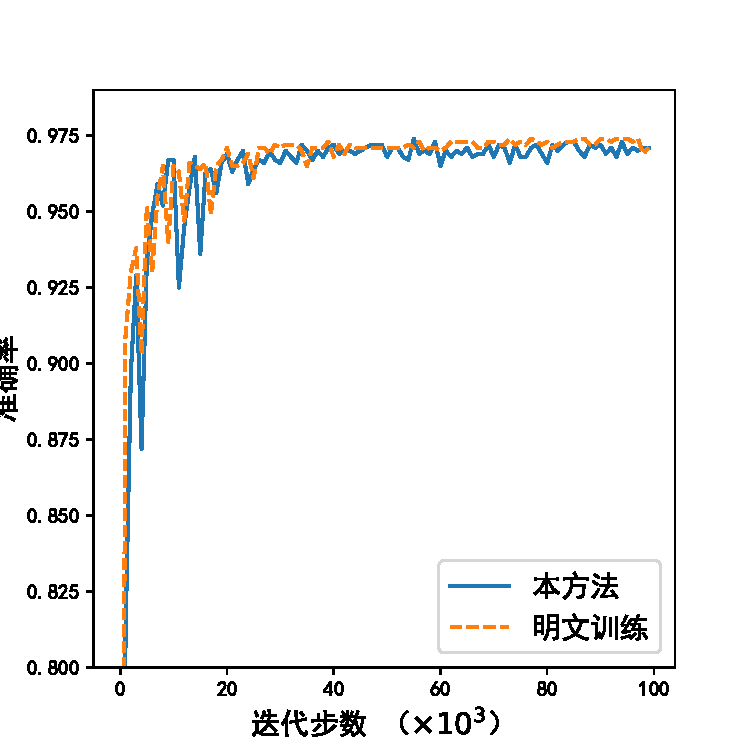
\includegraphics[width=\linewidth]{Z_Resources/ss-perm_lr.pdf}
    \caption{Gisette数据集逻辑回归训练曲线}
    \end{subfigure}
    %
    \begin{subfigure}[b]{0.47\linewidth}
    \centering
    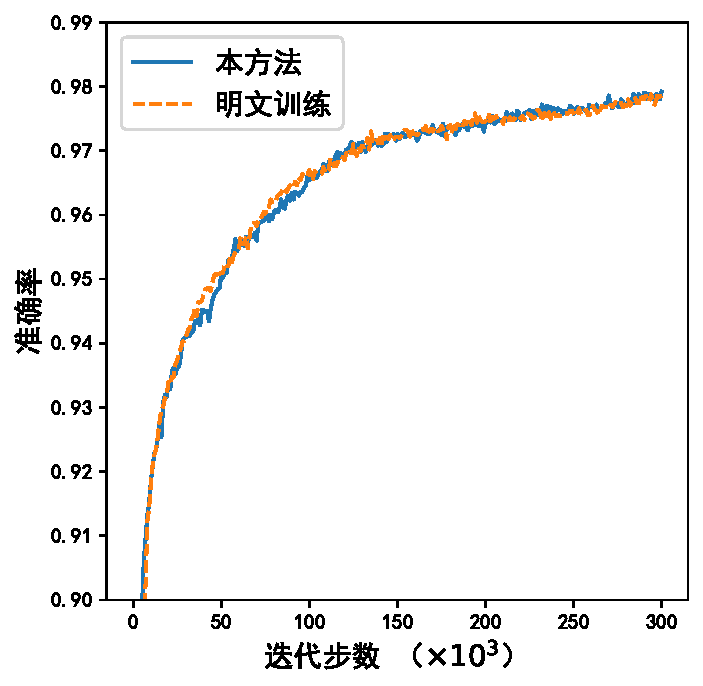
\includegraphics[width=\linewidth]{Z_Resources/ss-perm_dnn1.pdf}
    \caption{MNIST数据集DNN1训练曲线}
    \end{subfigure}
    
    \begin{subfigure}[b]{0.47\linewidth}
    \centering
    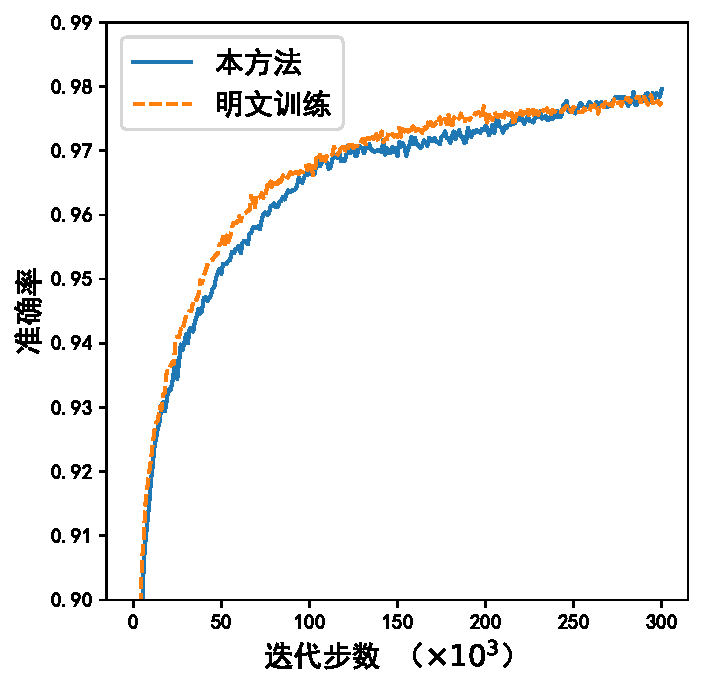
\includegraphics[width=\linewidth]{Z_Resources/ss-perm_dnn2.pdf}
    \caption{MNIST数据集DNN2训练曲线}
    \end{subfigure}
    %
    \begin{subfigure}[b]{0.47\linewidth}
    \centering
    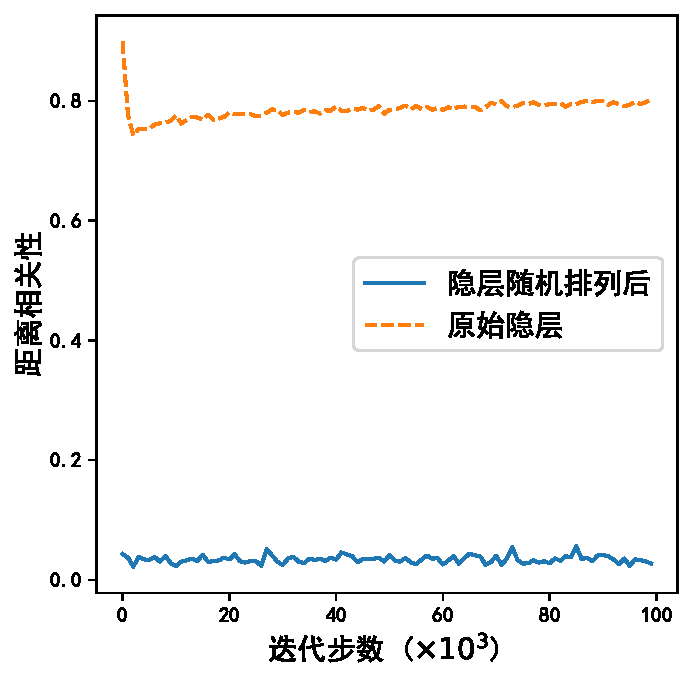
\includegraphics[width=\linewidth]{Z_Resources/ss-perm_dnn1-dcor.pdf}
    \caption{MNIST数据集DNN1隐层距离相关性}
    \end{subfigure}
\caption{在Gisette和MNIST数据集上的训练结果}
\label{fig:ss-perm:train}
\end{figure}

\subsubsection{隐层隐私泄漏情况}
我们在\autoref{fig:ss-perm:train}c中展现了DNN1隐层与输入的距离相关性,以及本方法暴露的数据(随机排列后的隐层)与输入的距离相关性。
%
可以看出,隐层与输入的距离相关性较高,在整个训练过程中维持在0.8左右的水平。
而随机排列后的隐层数据,其距离相关性大幅度降低到0.1以下,表明随机排列后的数据几乎不会带来隐私泄露。
%


另外,我们也测试了MNIST数据集中,基于隐层表征查找相似样本的结果。
%
为了考察在特殊情况下的安全性,提高隐私保护的难度,我们令一批样本全部为同一类别,因此随机排列并不能引入其他类别样本的信息。
%
实验结果呈现在\autoref{fig:ss-perm:permutation-attack}中。
%
其中最左边的列表示原始样本,蓝色方框表示框内的样本被合并为单个向量来进行随机排列。


\begin{figure}[h!]
    \centering
    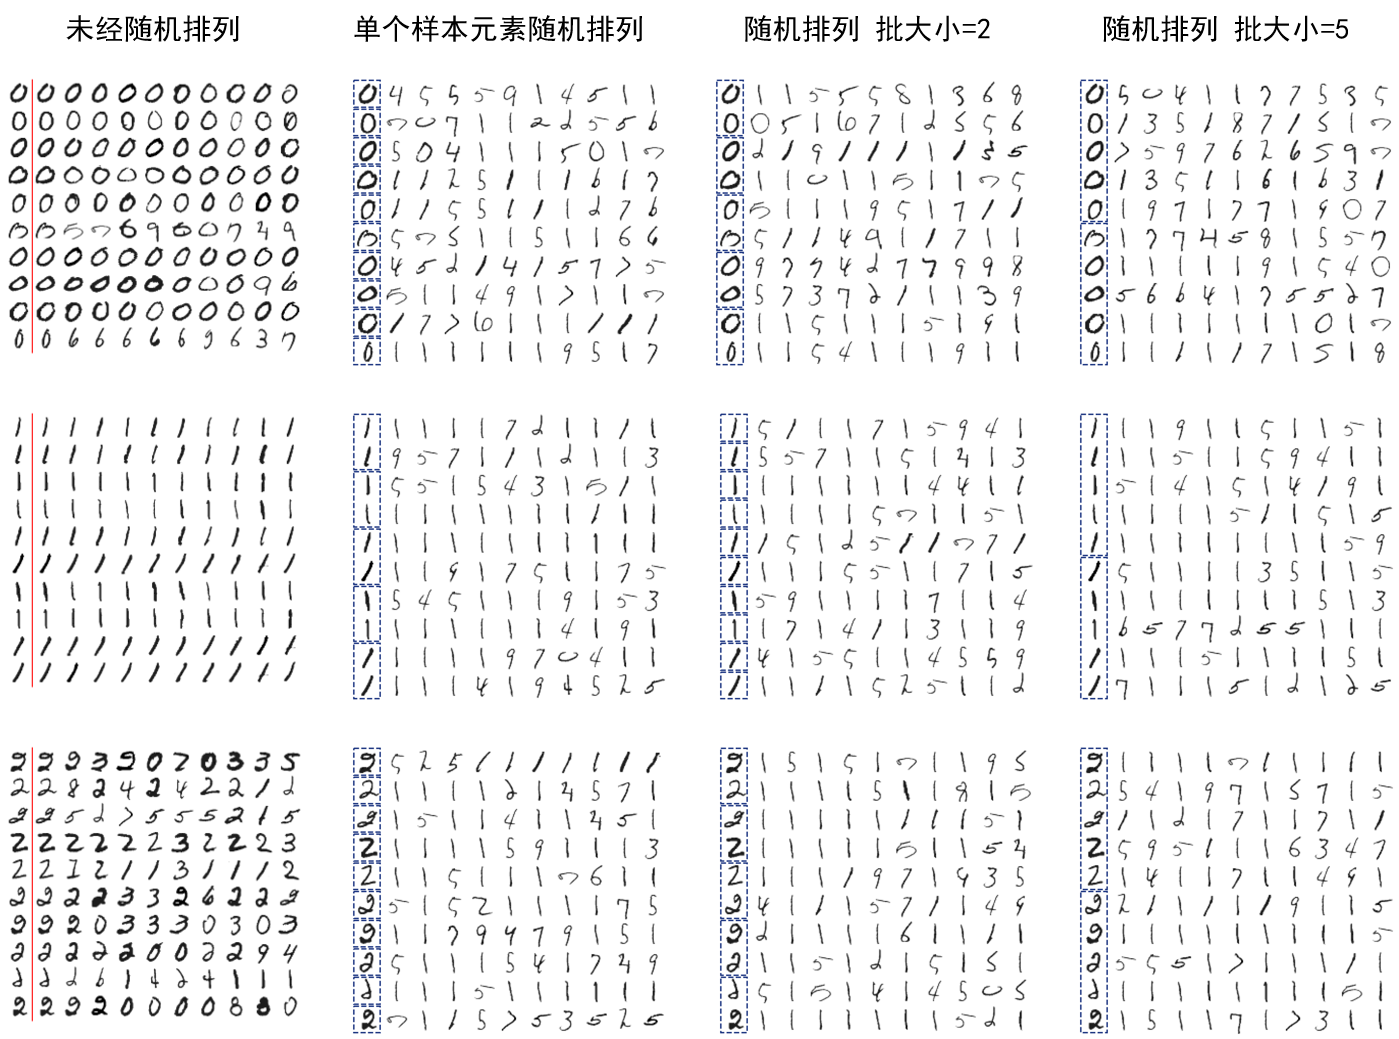
\includegraphics[width=\linewidth]{Z_Resources/ss-perm_permutation-attack.png}
    \caption{隐层表征随机排列前后的相似样本示意图}
    \label{fig:ss-perm:permutation-attack}
\end{figure}

实验结果表明,如果没有进行随机排列,也就是直接暴露隐层表征时,攻击者很容易根据隐层表征找到相似的样本。
%
而采用了随机排列之后,则攻击者找到的相似样本和原始样本无关。
%
无论原始样本属于哪个类别,找到的相似样本都是一些笔画较细的“1”等图像。
%
这是因为两个隐层表征$\bvec x, \bvec y \in \mathbb R^d$之间的距离可以用表示为
$\mathbb E_i [(x_i - y_i)^2] = \mathbb E_i [x_i^2 + y_i^2 - 2x_i y_i]$。
%
当$\bvec x, \bvec y$归一化后且$x_i, y_i$之间没有相关性时,则上式可以进一步表示为
$\mathbb E_i [x_i^2] + \mathbb E_i [y_i^2]$。
%
注意到$x_i, y_i \ge 0$。
%
因此,若$\mathbb E_i [y_i^2]$越小,就会导致$\mathbb E_i [(x_i - y_i)^2]$越小。
%
而较小的$\mathbb E_i[y_i^2]$对应是分布更加集中的$\bvec y$,其输入大概率是黑色像素较少的图片,因为MNIST数据集的图像以白色部分为主。
%
